\documentclass[../main.tex]{subfiles}

\begin{document}

A background to the plasma state of matter, including a definition of plasma, characteristics and important equations used in this research, and a background to plasma spectroscopy.
\section{Definition of plasma}
Plasma is defined \cite{Chen1984IntroductionFusion} as an ionized gas of charged and neutral particles, which satisfies the \emph{quasi--neutrality} condition. An example of a non--neutral plasma is a beam of charged particles. Yet, a plasma cannot be treated simply as an ordinary gas which is electrically conducting. The particles that carry charge generate electromagnetic fields that are regarded as properties of the plasma. Due to the long range of the inter-particle forces each charged particle in a plasma interacts with a large number of other charged particles resulting in \emph{collective behaviour}.

Inside such a medium diverse collective phenomena can occur which ultimately allow for electron acceleration in laser-driven plasma wakefields.

To better understand this definition, we present two main characteristics of plasma behavior in space (Debye length) and time (plasma oscillations).

\subsection{Debye shielding length}\label{sec:debye}
The Debye length determines the effective interaction between charged particles in a plasma. The potential field $\phi$ around a charged particle is effectively screened by the cloud of the other charged particles; its force range is now confined within a certain characteristic length, $\lambda_D$, called the Debye shielding length, determined by the density and the temperature of the plasma:
\begin{equation}
\phi(r)=\frac{q_i}{4\pi\varepsilon_0 r}\exp{\left(-\frac{r}{\lambda_D}\right)},
\end{equation}
where
\begin{equation}
\lambda_D=\sqrt{\frac{\varepsilon_0 k_B T_e}{n_e e^2}}=\sqrt{\frac{k_B T}{m_e}}\frac{1}{\omega_p}.
\end{equation}
For a plasma with characteristic thermal energy of \SI{1}{\electronvolt}, number density $n_e \sim \SI{e18}{\per\cubic\cm}$, we get $\lambda_D \sim \SI{7}{\nm}$.
For any volume with a length scale $L$ satisfying 
\begin{equation}
L \gg \lambda_D,
\label{eq:quasiNeutrality}
\end{equation}
overall quasi-neutrality is a good approximation. This inequality is the first criterion for the definition of a plasma. If $L\lesssim \lambda_D$, then our approximations break down and significant deviations from quasi-neutrality occur.
\subsection{Plasma Oscillation}\label{ssec:oscillation}
The transfer of electrons from a given region of space to a neighbouring region induces a charge separation. This local charge gives rise to an electric field $E$. Since the electrons are much lighter than the ions, they respond much more rapidly to the electric field, and the motion of the ions can be neglected in first instance. The electric field pulls the electrons back to their initial position in order to reduce the local charge separation which is the source of the electric field. Those electrons produce another non-equilibrium distribution in the opposite direction, and so on, performing an oscillatory motion, with the Coulomb force acting as the restoring force and the mass of the electron as the inertia. This is called a plasma oscillation\sidenote{Eq. \ref{eq:plasma-frequency} for $\omega_p$ does not depend on $k$, so the group velocity $\mathrm{d}\omega / \mathrm{d}k$ is zero - the disturbance does not propagate.}, defined as
\begin{equation}
		\omega_p=\sqrt{\frac{n_e e^2}{m_e \varepsilon_0}}\si[per-mode=fraction]{\radian\per\sec}.\label{eq:plasma-frequency}
\end{equation}
For a typical plasma density of $n_e \sim \SI{e18}{\per\cubic\cm}$, we get \\ $\omega_p=\SI{5.6e13}{\radian\per\sec}$, which lies in the microwave range.

\subsection{Collective behaviour criteria}
A measure for the average number of particles with density $n_e$ inside a sphere of radius $\lambda_D$ is called the Debye number, $N_D$, via which the (dimensionless) plasma parameter $\Lambda$ is defined:
$$
    N_D=\frac{4\pi}{3}n_e \lambda_D^3=\frac{\Lambda}{3},
$$
\begin{equation}
    \Lambda=4\pi n_e \lambda_D^3 \propto \frac{T^{3/2}}{\sqrt{n_e}}.
\end{equation}
Collective behaviour for plasmas in LWFA environments requires, therefore two criteria: overall quasi-neutrality (eq. \ref{eq:quasiNeutrality}), and hot plasma, yet not too dense: $\Lambda \gg 1$.


\section{The spectrum of Hydrogen and Stark Broadening}\label{sec:hydrogen}
The emission spectrum of atomic hydrogen, due to the electron making a transition between two energy levels, has been divided into a number of spectral series, with wavelengths that can be given by the Rydberg formula. Transitions to the first excited state ($n_f=2$) are known to spectroscopists as the \textit{Balmer series} \sidenote{The others, to name a few, are Lyman ($n_f=1$) and Paschen ($n_f=3$).}, denoted historically as H\textsubscript{$\alpha$}, H\textsubscript{$\beta$}, H\textsubscript{$\gamma$} and so on, where H stands for the element Hydrogen. It is convenient to observe H\textsubscript{$\alpha$} ($n_i=3 \to n_f=2$, \SI{656.23}{\nm}) and H\textsubscript{$\beta$} ($n_i=4 \to n_f=2$ ,\SI{486.13}{\nm}) because both fall in the visible region.

Spectroscopy study of such emission can give information about the physical conditions in the plasma, such as density and temperature. Spectroscopic techniques have the advantage over some other methods -- those involving probes, for example -- that they do not interfere in any way with the plasma. An inherent shortcoming of such observation is the fact that radiation is collected only along the line of sight in the direction of observation and any local information is therefore lost \cite{Thorne1988Spectrophysics}.

The observed intensity of the radiation emitted depends on \cite{McWhirter1965PlasmaTechniques}
\begin{enumerate}[label=(\alph*)]
\item The probability that there is an electron in the upper level of the transition
\item The atomic probability of the transition in question, designated by $A_{i\to j}$ for a transition from level $i$ to level $j$.
\item The probability of the photons thus produced escaping from the volume of the plasma without being reabsorbed.
\end{enumerate}
In many cases it is possible to neglect the last process (c) and use the approximation of optically thin plasma \cite{McWhirter1965PlasmaTechniques} (explained in the next paragraph). The calculation of the transition probability (process (b)) is a matter of atomic physics, for which numerical values are tabulated.% It is the first process that we concentrate on here presenting a plasma model to perform plasma diagnostics.
\begin{description}
  \item[\textnormal{Optical depth}] \hfill \\ For a beam of intensity $I$ transferring through a plane--parallel element of medium (plasma in our case) of thickness $z$, the optical depth $\tau$ (dimensionless) is a measure of the opacity of the element:
\begin{equation}
    \tau=-\kappa z
\end{equation}
Here $\kappa$ is the linear absorption coefficient (\si{\per\cm}). In this simple case, the emergent and incident intensities $I_\text{out}$ and $I_\text{in}$ are related by \marginnote{Equation \ref{eq:radiative-transfer} is the simplest equation of radiative transfer.}
\begin{equation}
    I_\text{out}=I_\text{in}e^{-\kappa z}.
    \label{eq:radiative-transfer}
\end{equation}
Media with optical depths less than unity and exceeding unity, are called optically \emph{thin} and optically \emph{thick}, respectively. I.e., by optically thin plasma, we mean that the freely propagating radiation is not significantly attenuated by the plasma environment and reaches the detector without re--absorption.
\end{description}

The appropriate plasma model for density and temperature measurements in the present discussion is that of \emph{local thermodynamic equilibrium} (LTE):

In an isolated, closed system where the radiation and matter have reached equilibrium (black body cavity, for example), the distribution of the kinetic motions, level populations and radiation fields are described by some known, well--defined functions of a single parameter --- the system temperature. This situation, called \textit{thermodynamic equilibrium}, serves as a starting point for systems that are not in thermodynamic equilibrium.

In general, the various "temperatures" --- kinetic temp' (via Maxwell--Boltzmann distribution) for the thermal motions , excitation temp' (via Boltzmann factor) for the level populations and radiative temp' (via Planck's relation) for the radiation field would be different from each other, and become the same only for a system in thermodynamic equilibrium. If the level populations were controlled by a single physical mechanism, either collisions or radiative process, their distributions would approach the above mentioned thermodynamic limit. This follows from the principle of detailed balance, or microscopic reversibility, which states that each energy exchange process must be balanced by its exact inverse: For every photon emitted a photon of the same frequency must be absorbed, for every excitation by electron collision there must be a  de--excitation between the same two levels, etc.

%In what follows we will assume that in a small neighbourhood (element of volume) of any point in the system, there is an equilibrium situation described by a local Maxwell-Boltzmann distribution function. For larger spatial scales there may exist gradients of $T$ but these scales are so large that locally the equilibrium is not perturbed; time variation of $T$ may exist, but on such slow time scale that instantaneous equilibrium is a very good approximation.

The assumption of LTE is a very powerful one, since it allows us to use the familiar results of statistical mechanics and thermodynamics  for ionization equilibrium $A^{+} +e\Leftrightarrow A$.

Continuum radiation from the LTE model plasma arises from the interaction of initially free electrons with the positive ions or atoms that are present.

\textbf{Classification of Radiation Transitions}
The contributions to the spectrum emitted by a plasma are classified according to their type --- continuum or line radiation \cite{Thorne1988Spectrophysics}:
\begin{marginfigure}
    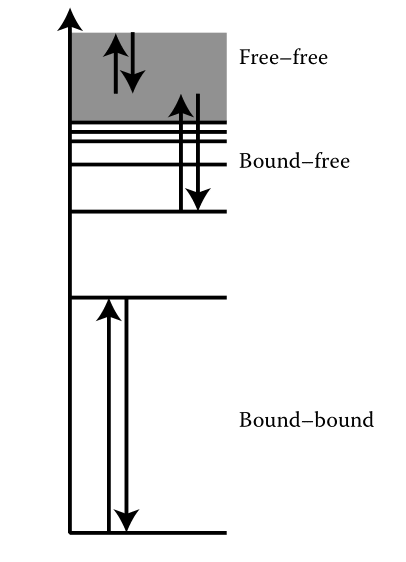
\includegraphics[width=\marginparwidth]{figures/electron-transitions.png}
    \label{fig:electron-transitions}
    \caption{Energy levels and electron transitions induced by electron--ion interaction. From Plasma Physics and Engineering Fridman and Lawrence}
\end{marginfigure}
\begin{enumerate}
    \item Free--free transition. Both initial and final electron states are in continuum. A free electron in this transition loses part of its kinetic energy in the Coulomb field of a positive ion due to deflection. The emitted energy in this case is a continuum, usually infrared and called bremsstrahlung. The principle of detailed balance requires the existence of the inverse bremsstrahlung process: absorption of radiation by a free electron and ion.
    \item Free--bound transition. Electron transition between a free state in continuum and a bound state in atom. This transition accounts for energy emitted when electrons recombine with ions and the reverse process of photoionization. The emitted energy in this case is a continuum, too.
    \item Bound--bound transition. Electron transition between discrete atomic levels, results in emission (and absorption) of spectral lines. %Energy emitted in this case is that of spectral lines.
\end{enumerate}
If the free electrons are distributed among the energy levels available to them, then, according to statistical mechanics, their velocities have a Maxwellian distribution. Thus the number of electrons of mass $m_e$ and velocities between $v$ and $v+\mathrm{d}v$ is
\begin{equation}
\mathrm{d}N_v=4\pi N_e\left( \frac{m_e}{2\pi k_B T_e} \right)^{3/2} \exp\left(-\frac{m_e v^2}{2k_B T_e}\right) v^2 \mathrm{d}v.
    \label{eq:maxwellian}
\end{equation}
For the bound levels the distributions of population densities are given by the Boltzmann and Saha equation, viz.,
\begin{equation}
		\frac{N_\text{i}}{N_\text{j}}=\frac{g_\text{i}}{g_\text{j}}e^{\frac{E_i-E_j}{k_B T}}
		\label{eq:boltzmann}
		%=\frac{g_i}{g_j}e^{-\frac{h\nu_{ij}}{k_B T}}
\end{equation}
where $g_{i,j}$ are the degeneracies of the states, and
\begin{equation}
		\frac{N_\text{e} N_\text{i}}{N_\text{a}}=\frac{g_e g_i}{g_a} \left(\frac{2 \pi m_e k_B T}{h^2}\right)^{3/2}e^{-U_i/k_B T},
		\label{eq:saha}
\end{equation}
where $U_i$ is ionization potential, $g_a$, $g_i$ and $g_e$ are the degenaracies of the atoms, ions and electrons; $N_\text{a}$, $N_\text{i}$ and $N_\text{e}$ are their number densities.

The three equations, \ref{eq:maxwellian}--\ref{eq:saha}, describe the state of the electrons in an LTE model plasma \cite{McWhirter1965PlasmaTechniques}.

% widths, shapes and intensities of spectral lines depend on the temperature, pressure and electron density of the environment of the atom or molecule, as well as on its intrinsic properties. If the broadening and other physical processes are properly understood and the necessary atomic parameters are known, the spectral lines can give information about the physical conditions in the emitting or absorbing gas or plasma.

All transitions emit spectral lines that have finite width. The observed lineshape function $f(\lambda)$ and its width $\Delta \lambda_{1/2}$ depend on the temperature and pressure of the emitting plasma. If the broadening and other physical processes are properly understood and the necessary atomic parameters are known, the spectral lines can give information about the physical conditions in the emitting plasma \cite{Thorne1988Spectrophysics}. The dominant cause of line broadening in plasma is the inter--atomic Stark effect \cite{Wiese1965PlasmaTechniques}. In our plasma conditions, the measurement of Stark half--widths has emerged as one of the most reliable and convenient methods for the determination of electron densities \cite{Wiese1965PlasmaTechniques}.


%In the state known as LTE it is possible to find a common temperature, which may vary from place to place, that fits the Boltzmann and Saha distributions and also the Maxwell distribution for the velocities of the electrons.

% when presenting this argument, cite Thorne stating this:
% In real situations there is often an equilibrium distribution of one or more, but not all, of these forms of energy, and the temperature parameter T may vary from one to another. >>For example, in a  low-pressure discharge tube the gas kinetic temperature may be a  couple of orders of magnitude smaller than the Boltzmann temperature, while the spectrum bears no resemblance to a  black-body continuum at any temperature.<< The form of energy most likely to be out of balance with the others is the radiation energy.
%The distribution of population densities of the energy levels of the electrons is the same as it would be in a system in complete thermodynamics equilibrium.
%This model holds when the system is in detailed balance.


As stated previously, plasma is a charged medium, and this leads to a broadening of the lines named \textit{Stark Broadening}\sidenote{Classified under \textit{Pressure broadening} mechanism.}: When the density of charged particles in a plasma is sufficiently large, their electric micro--fields perturb the atomic energy levels \cite{Griem1974SpectralPlasmas.}; An emitting atom at a distance $r$ from an ion or electron is perturbed by an electric field $E=e/(4\pi \varepsilon_0 r^2)$, and the interaction between the atom and the field is described by the Stark effect. A perturbation proportional to $E$ exists only in the case of the hydrogen atom or hydrogen--like atoms; for all other atoms the first non-vanishing interaction is the quadratic Stark effect\cite{Thorne1988Spectrophysics}, proportional to $E^2$ and thus to $1/r^4$.

The line shape for the Stark broadening assumes that of a Lorentzian \cite{Wiese1965PlasmaTechniques,Hutchinson2002PrinciplesDiagnostics},
\begin{equation}
I\left( \lambda \right)=\frac{A^2}{4\left( \left(\lambda-\lambda_0\right)^2+\Delta \lambda_{1/2}^2\right)}. \label{eq:Stark_Broadening}
\end{equation}
where $\Delta \lambda_{1/2}\left[\si{\nm}\right]$ is the full width at half maximum for a profile centered at wavelength $\lambda_0$.

This phenomenon for hydrogen lines is very well understood, and the dependence of the line width on the plasma concentration and plasma density has been tabulated \cite{Griem1964PlasmaSpectroscopy,Griem1974SpectralPlasmas.}, but, from the theoretical point of view, there does not exist any model that enables accurate calculations of Stark broadening over a large electron density range\cite{Griem2000StarkPlasmas}. 

The following equation relates electron density to the width of the emission line for the H\textsubscript{alpha} line:
\begin{equation}
n_e=\left( \frac{\Delta\lambda_{1/2}}{\gamma\left(n_e,T_e\right)}\right)^{3/2}.
\end{equation}
$\gamma\left(n_e,T_e\right)$ may be evaluated numerically and experimentally\cite{Griem2005ComparisonResults}, the dependence of which on the plasma density and temperature is rather weak and it has been neglected in our measurements, at which the following was used:
\begin{equation}
n_e=\left( \frac{\Delta\lambda_{1/2}\left[\si{\nm}\right]}{5.4}\right)^{3/2}. \label{eq:delta_lambda}
\end{equation}

%\section{Paschen Curve}\label{sec:paschen}
%Paschen's Law states that the breakdown voltage is a unique function of the product of gas pressure $p$ and the gap length $d$ for a particular gas. The curve is shown in figure %\ref{fig:paschen_curve}.
%\begin{marginfigure}
    %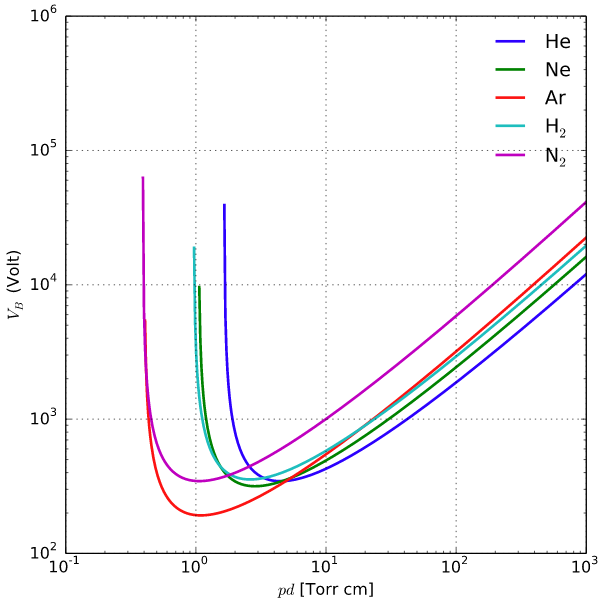
\includegraphics[width=\marginparwidth]{figures/paschen_curve.PNG}
    %\label{fig:paschen_curve}
    %\caption{Paschen curve --- voltage versus the pressure--gap length product.}
%\end{marginfigure}

\section{Plasma acceleration, laser wake--field acceleration}\label{sec:wakefield}
Laser--driven plasma-based accelerators were originally proposed by T. Tajima and J. Dawson in 1979 \cite{Dawson1979}, on purpose for experiments on nuclear physics and the structure of matter. Conventional radio--frequency linear accelerators (linacs) begin to approach their limit, because the accelerating electric fields  must  be  less  than  $\SI{100}{\MV\per \m}$  to  avoid material breakdown. This limits the highest energies achievable through cost, as each \si{\GeV} of energy requires $\sim \SI{100}{\m}$ of acceleration length \cite{Esarey2009PhysicsAccelerators}.

If the limiting factor on the scale of the accelerator is ionisation of the material, then an attractive alternative with reasonably sized facilities is to use plasma as the medium for the acceleration mechanism.

In a plasma accelerator, a longitudinal electron plasma wave (wakefield) is formed and electrons injected into the plasma near the high--density area will experience an acceleration toward it by the plasma. This method, termed \emph{Laer WakeField Acceleration} (LWFA), utilizes an ultrashort ($\sim\SI{100}{\fs}$), high--power (\si{\TW}) laser that provides a large electric field because of charge separation. Plasma formed by initiating a discharge in a narrow channel made within a tube (i.e., \textit{discharge capillary}) satisfies promising conditions for a plasma source to exploit LWFA, on a length scale of centimeters \cite{Gonsalves2019PetawattWaveguide,Leemans2014Multi-GeVRegime}. The injected electrons' acceleration continues as the wakefield travels through the plasma waveguide. The research has widely grown since the mid 1980s, when ultrashort laser pulses of sufficient energy became available after the damage threshold inherent in optical amplifiers had been overcome by means of Chirped Pulse Amplification (CPA) \cite{Strickland1985CompressionPulses}.
\begin{figure}
    \centering
    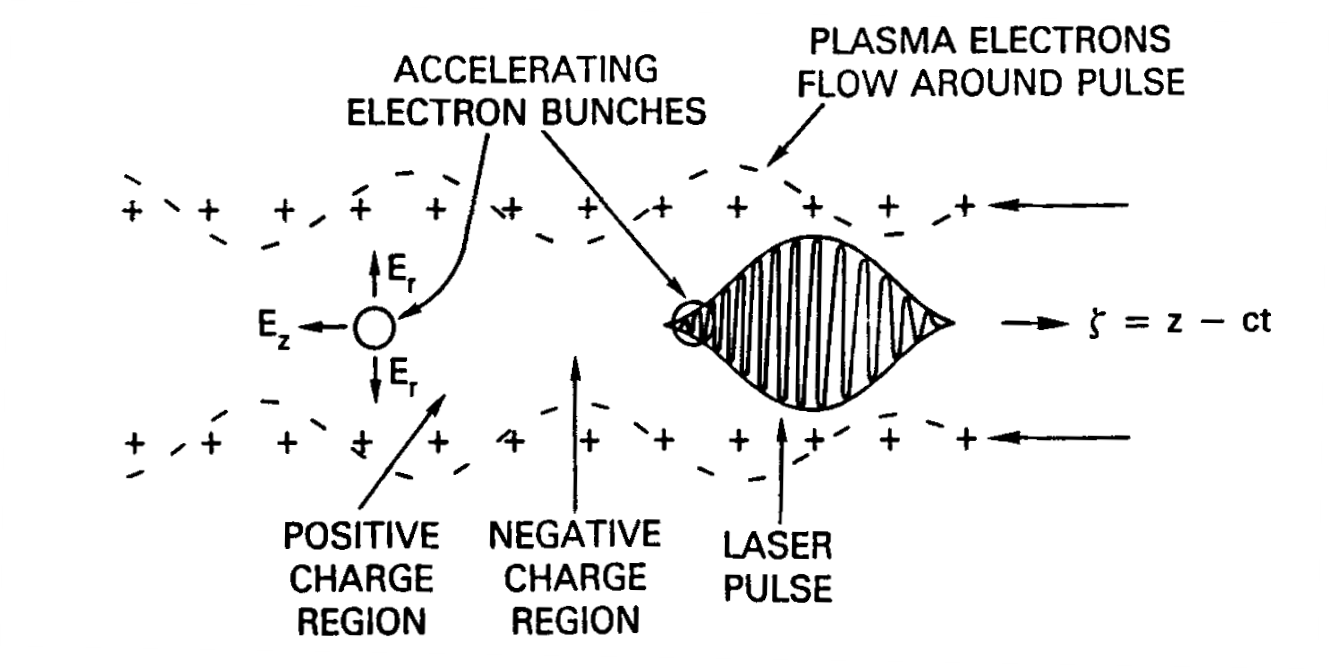
\includegraphics[width=\textwidth]{figures/lwfa_schematic.PNG}
    \caption{Adapted from \href{https://aip.scitation.org/doi/pdf/10.1063/1.37621}{here}.}
    \label{fig:lwfa-schema}
\end{figure}

%It is necessary to provide transportation of the laser pulse in an underdense(\textcolor{red}{?}) plasma over distances on the order of the acceleration length $l_\text{acc}$,
%\begin{equation}
%    l_\text{acc}\approx\frac{c}{\omega_p}\left(\frac{\omega_0}{\omega_p}\right)^2
%\end{equation}
%Here, $\omega_0$ is the  carrier frequency of laser radiation.

To date, two major limitations of LWFA prevent quality electron beams from reaching high energies \cite{Esarey2009PhysicsAccelerators}. The former regards to the laser pulse that creates the wake, and the latter to the acceleration of the charged particles:
\begin{description}
  \item[\textnormal{Defocusing of the laser radiation}] \hfill \\ It is necessary to provide transportation of the wake--driving laser without significant transverse spreading when propagating within the plasma. In the absence of some form of optical guiding, the wake would propagate over a distance of the order of the Rayleigh length, $z_R$\sidenote{$z_R=\pi w_0^2/\lambda$, where $\lambda$ is the wavelength of laser light. $w_0$ is defined in eq. \ref{eq:beamParameters}.}. Therefore, conditions should be created for both focusing of laser radiation to a small spot of radius $r_0$, together with transportation of the laser pulse over many Rayleigh lengths without diffraction spreading.
  \item[\textnormal{\label{dephasing-length}Electron dephasing length}] \hfill \\ The dephasing length is the distance over which an ultra relativistic electron outruns the wakefield of the radiation pulse and no longer gains energy \cite{Esarey2009PhysicsAccelerators,Sprangle1988LaserGuiding}. Multiple acceleration stages, all sequentially phase synchronized, have been proposed to overcome the propagation distance limitation \cite{Esarey2009PhysicsAccelerators}.
\end{description}

We will now give a short explanation about the geometry of Gaussian beams and plasma waveguides as a method to tackle the defocusing of the laser radiation, and then present a proposed scheme to overcome the dephasing length.

\subsection{Plasma waveguides}
Although the divergence of a real laser beam can sometimes be negligible, this is not the case here because the intensities feasible for plasma accelerations can only be achieved by focusing the laser beam to a tiny spot of a few tens of microns in diameter. Such a beam will rapidly diverge in any homogeneous medium. The divergence is conventionally characterized by the Rayleigh length, defined to be the distance over which the intensity of the beam falls by a factor of 2 with respect to that in the focal plane. See figure \ref{fig:typical-beam}.
\begin{marginfigure}
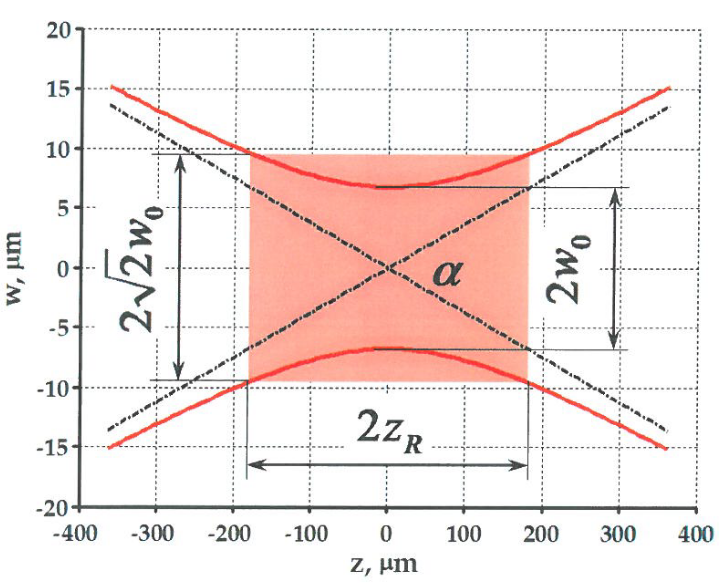
\includegraphics[width=\marginparwidth]{figures/beam-geometry.PNG}
\caption{Typical beam geometry around the focal point.}
\label{fig:typical-beam}
\end{marginfigure}
It can be shown \cite{Saleh2019BeamOptics}, that for a beam of initial diameter $D$ focused by a parabolic lens with focal length $f$, the Rayleigh length and the waist radius are
\begin{equation}
\begin{split}
z_R & = \frac{\lambda}{\pi} \cot^2\alpha = \frac{4f^2}{\pi D^2}\lambda
\\
w_0 & = \frac{\lambda}{\pi}\cot \alpha=\frac{2f}{\pi D}\lambda
\end{split}
\label{eq:beamParameters}
\end{equation}
where $\alpha$ is the divergence angle.

For example, a \SI{75}{\mm} beam in diameter of a \SI{800}{\nm} laser focused by a \SI{1}{\m} parabolic mirror will have the (doubled) Rayleigh length of about \SI{0.4}{\mm}, whereas the dephasing length of an electron accelerating in plasma wakefield is typically \SIrange{1}{3}{\cm}.

The problem of making a tightly focused laser pulse ($~$\SI{20}{\um} waist diameter) propagate over many tens of Rayleigh lengths without divergence can be solved by constructing a preformed plasma channel with radially increasing density. Such channels, also known as plasma waveguides, are analogous to polymeric fibers in that they both rely on the same phenomenon --- total internal reflection resulting from axially--peaked refraction index. The simplest fiber consists of a transparent core in which light is confined, and a cladding surrounding the core, with a refractive index smaller than that of the core. On the contrary, plasma waveguides are formed dynamically, their radial decrease of refraction index is continuous and results from the corresponding increase of the plasma density.
\subsection*{Preformed plasma channel as a waveguide}
The dispersion relation \cite{Chen1984IntroductionFusion} for an electromagnetic wave propagating in a plasma takes the form 
\begin{equation}
\omega^2=\omega_p^2+c^2 k^2.
\end{equation}

Written as an expression for the index of refraction $\tilde{n}=c/v_\phi = ck/\omega$,
\begin{equation}
\tilde{n}=\frac{c k}{\omega}=\sqrt{1-\frac{\omega_p^2}{\omega^2}}\approx1-\frac{\omega_p^2}{2\omega^2}=1-\frac{N_e}{2N_\text{cr}}, \label{eq:index_of_refraction}
\end{equation}
where
\begin{equation}
    N_\text{cr}=\frac{\omega^2\varepsilon_0 m}{e^2}=\frac{\pi}{\lambda^2 r_e}
\end{equation}
is the critical plasma density, and $r_e$ is the classical electron radius.

The plasma is called \textit{underdense} for $N_e < N_\text{cr}$, with $N_\text{cr}\\\sim\SI{1.7e21}{\per\cubic\cm}$ for an \SI{800}{\nm} laser.

Equation \ref{eq:index_of_refraction} thus shows explicitly that the refractive index $\tilde{n}$ peaks on the axis of a plasma channel if the density has there a minimum.

Interpreted another way, the plasma's less--than--unity refractive index suggests that a normal density profile (maximum on the axis) causes the laser beam to diverge into the walls. If an inverted density profile (minimum on the axis) can be created, however, the lens effect becomes converging; The radiation is focused and trapped by the plasma.

The dependence $N_e(r)$ is usually termed the "radial density profile" (RDP). In an ideal plasma waveguide, the radial density profile is parabolic\sidenote{Essentially a power expansion of $N_e(r)$ up to second order in $r$.} \cite{Sprangle1992PropagationPlasmas},
\begin{equation}
    N_e(r)=N_e(0)+\Delta N_e\left( \frac{r}{r_\text{ch}}\right)^2,
    \label{eq:rdp}
\end{equation}
and is of special practical interest, because it is capable of guiding a tightly focused laser pulse while keeping its spot radius constant \cite{Sprangle1992PropagationPlasmas,Esarey1997Self-focusingPlasmas}. Here $N_e(r)$ is the electron density at a distance $r$ from the axis of the beam and $\Delta N_e$ is the increase in the electron density at $r=r_\text{ch}$ compared to the axial value. See figure \ref{fig:rdp_parabola}. Such guiding is accomplished for some waist radius of the guided beam (the \textit{matched} radius $w_m$), which is related to the geometry of a parabolic RDP as follows \cite{Esarey1997Self-focusingPlasmas}\sidenote{The radius of a mismatched beam oscillates as the beam propagates through the channel \cite{Esarey1997Self-focusingPlasmas}.}:
\begin{marginfigure}
    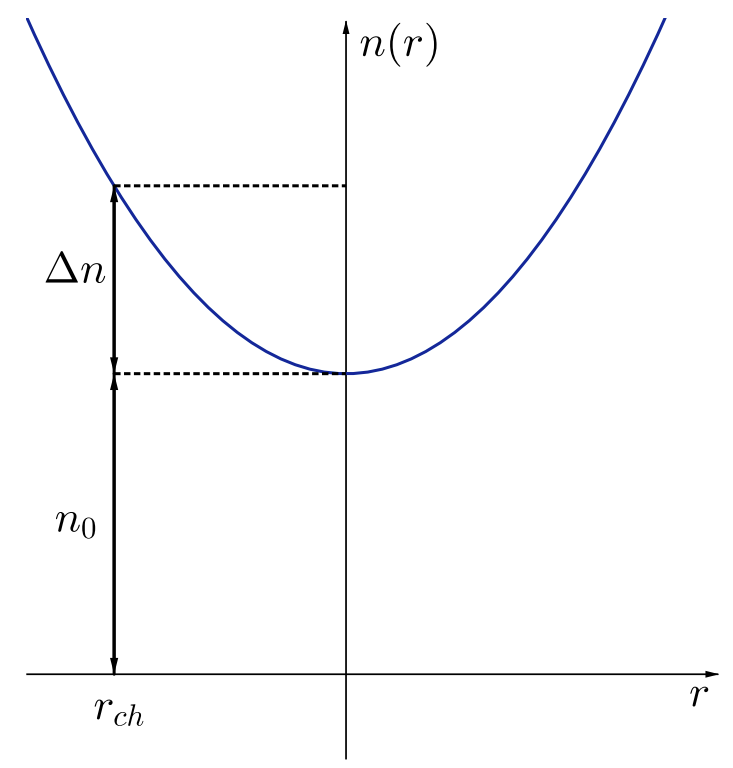
\includegraphics[width=\marginparwidth]{figures/rdp.PNG}
    \caption{Radial Density Profile}
    \label{fig:rdp_parabola}
\end{marginfigure}
\begin{equation}
    w_m=\left( \frac{r_\text{ch}^2}{\pi r_e \Delta N_e}\right)^{1/4}
    \label{eq:matched_radius}
\end{equation}
or, stated differently,
\begin{equation}
    w_m=\left( \frac{2}{\pi r_e n^{\prime\prime}(0)}\right)^{1/4}.
\end{equation}
In other words, it is the on-axis curvature of the RDP that defines the matched radius of the guided beam (if the obvious condition $r_\text{ch}>w_m$ is also satisfied).
Rearranging eq. \ref{eq:matched_radius} and substituting the numerical values of $\pi$ and $r_e$ leads to a practically convenient relation
\begin{equation}
    r_\text{ch}\left[\si{\um}\right]\approx0.09 w_m^2\left[\si{\square\um}\right]\sqrt{\Delta N_e\left[\SI{e18}{\per\cubic\cm}\right]}
\end{equation}
which means, in particular, that a minimal (absolute) depth of an RDP capable of waist-matched guiding of a beam with the waist radius $w_0$ is
\begin{equation}
\Delta N_\text{min}\left[\SI{e18}{\per\cubic\cm}\right]\approx\frac{113}{w_0^2\left[\si{\square\um}\right]}.
\end{equation}
For the beam geometry shown in figure \ref{fig:typical-beam} ($w_0\approx\SI{7}{\um}$) should be about \SI{2e17}{\per\cubic\cm}. % , i.e., is less but still of the same order as the optimal density at which a typical ultrashort laser pulse excites a plasma wake.
These conditions can be achieved in fully ionised plasma channels formed in capillary discharge  \cite{Butler2002GuidingWaveguide,Ehrlich1996GuidingExperiments}.



%\begin{marginfigure}
%    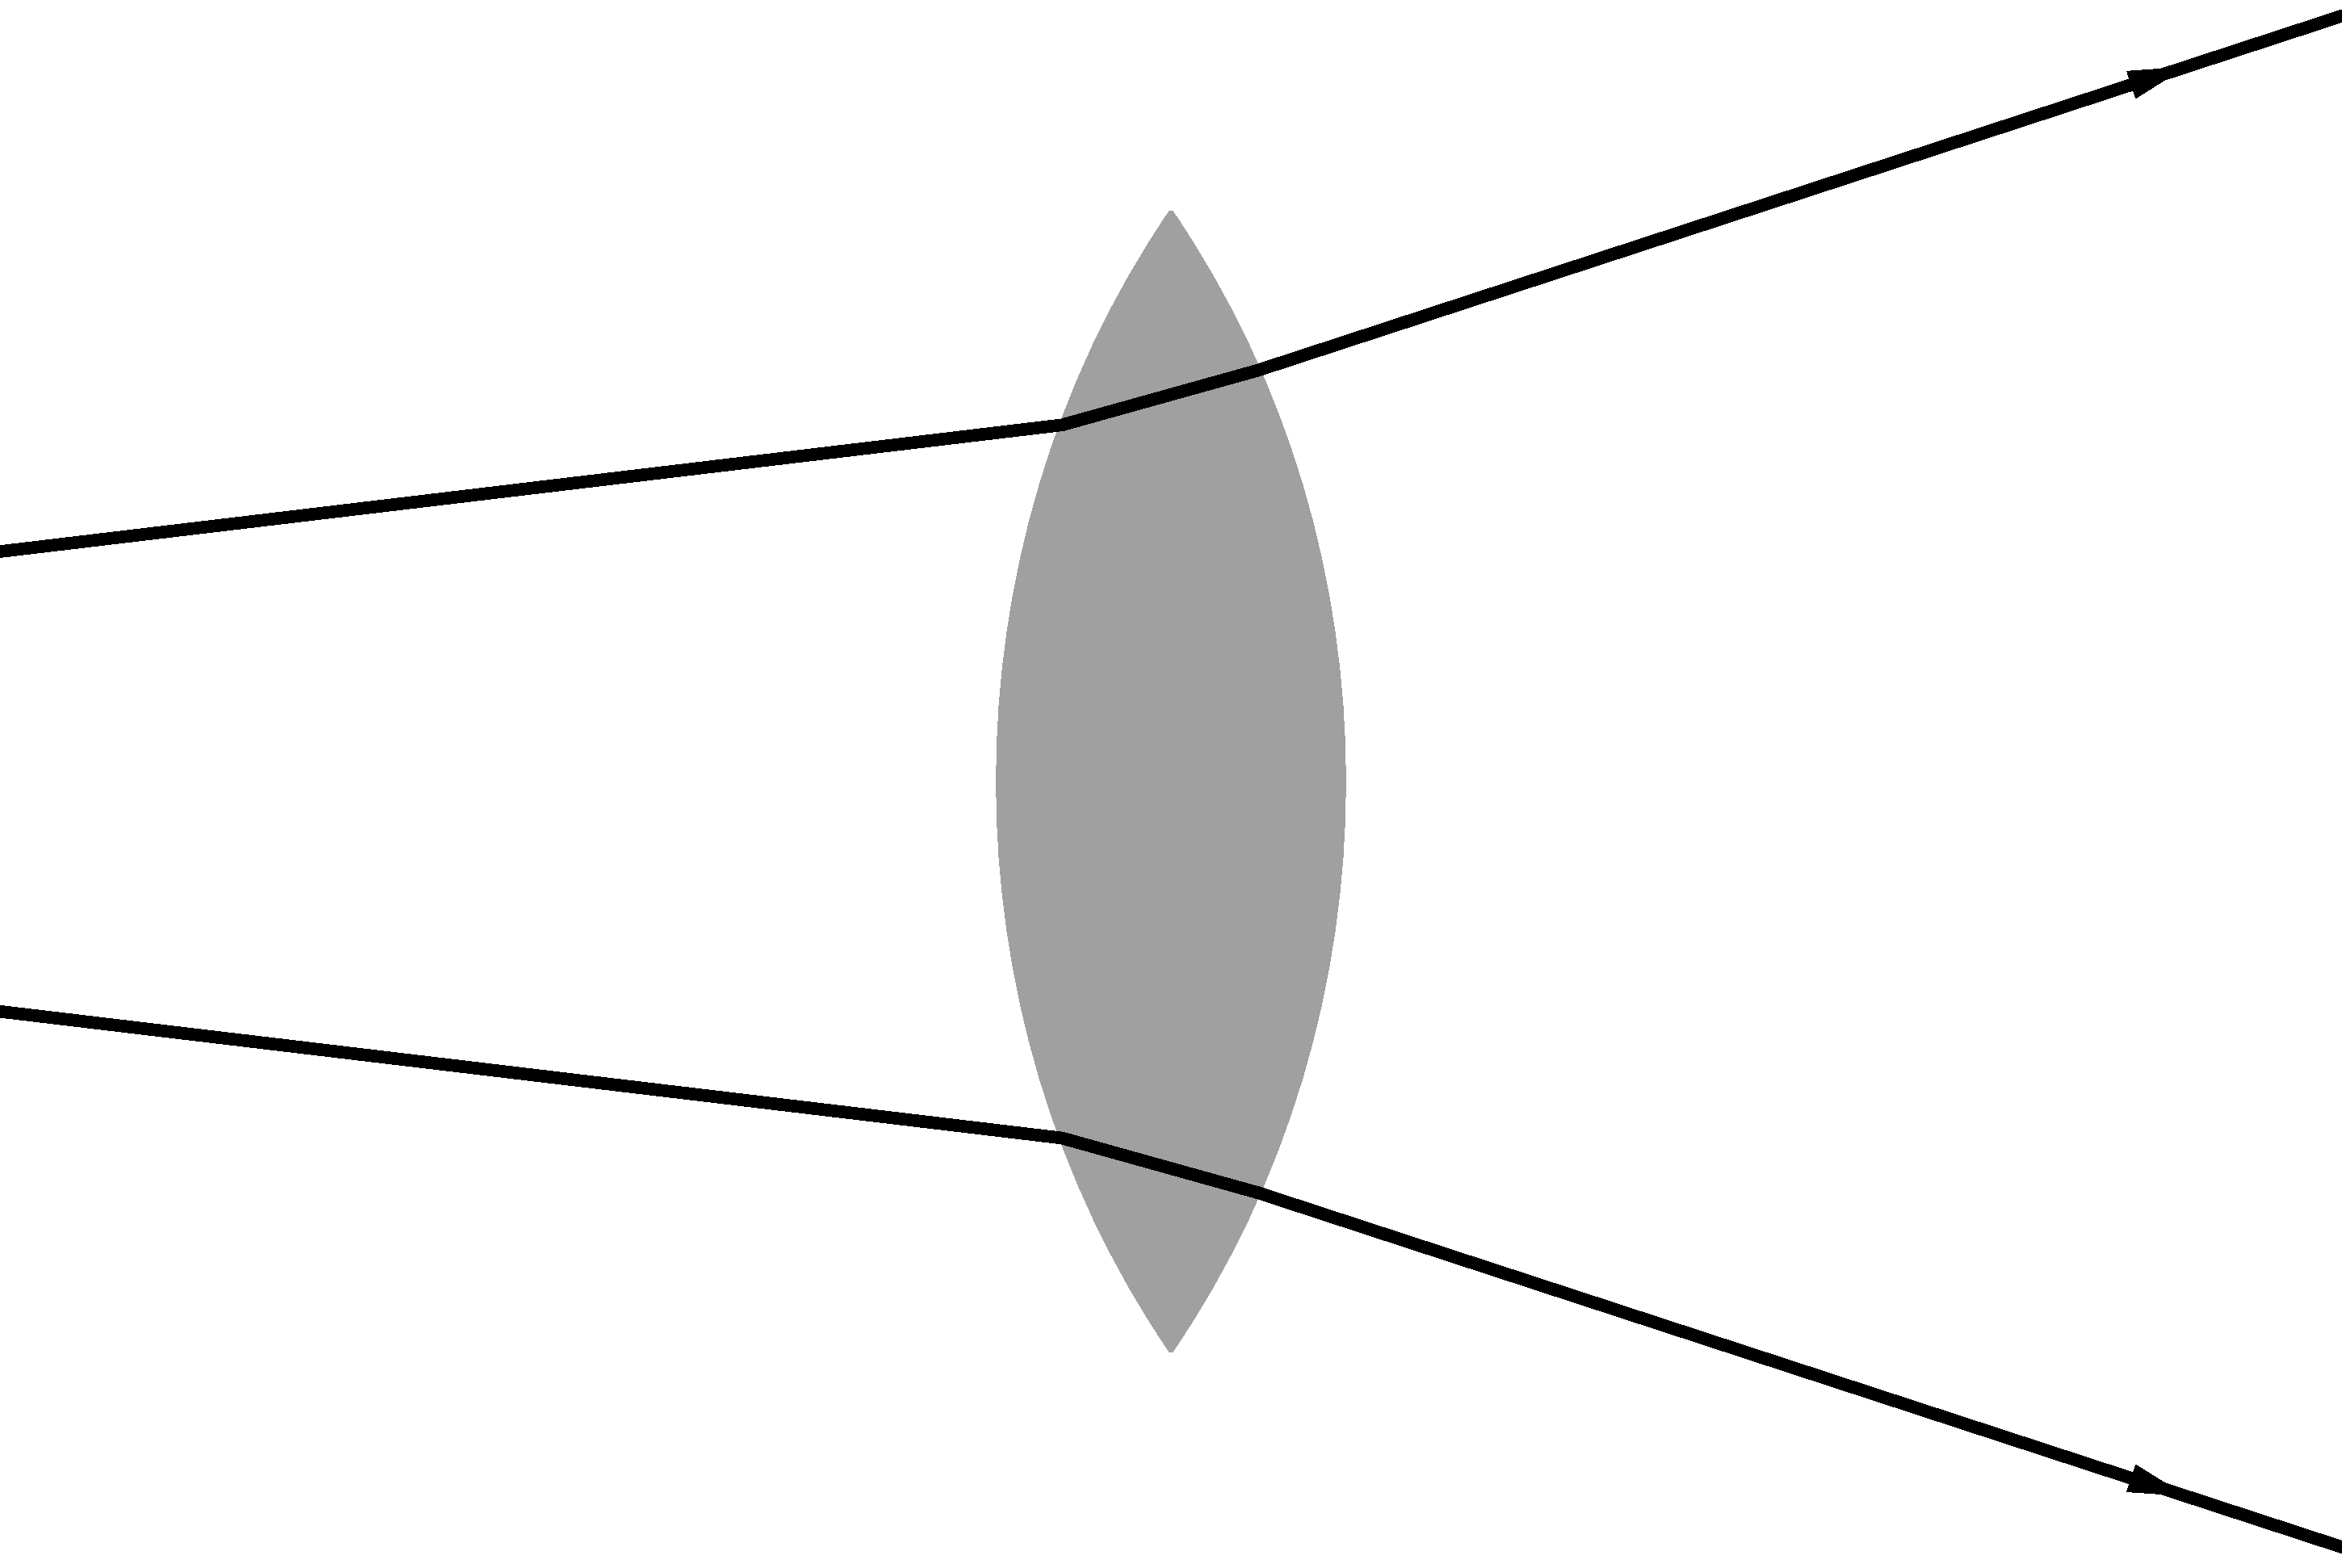
\includegraphics[width=\marginparwidth]{figures/chen4_30.pdf}
%    \caption{A plasma lens has unusual optical properties, since the index of refraction is less than unity.}
%    \label{fig:plasma_lens_chen}
%\end{marginfigure}


%A gas-filled capillary is an attractive technique to confine plasma \cite{Bobrova2002SimulationsWaveguide,Spence2001InvestigationWaveguide} and since the medium responsible for guiding is not damaged by the laser radiation, it is able to guide pulses with a wide range of intensities and wavelengths \cite{Dorchies1999MonomodeTubes}, and can prevent the diffraction spreading of the laser pulses \cite{Sprangle1990NonlinearPlasmas,Bulanov1994ShortChannel}.

\subsection{Multi--stage acceleration scheme}

As stated in page \pageref{dephasing-length}, in addition to defocusing, there is also the dephasing length: trapped electrons outrun or dephase the accelerating phase of the wakefield \cite{Esarey2009PhysicsAccelerators}. The current paradigm within the LWFA community envisions a \si{\TeV} LWFA composed of multiple $~$\SI{10}{\GeV} stages, which could be be optimized for efficiency, by matching the dephasing length to the depletion length of the laser pulse \cite{Schroeder2010PhysicsColliders}, thus using multiple LWFA stages to successively accelerate one electron beam to higher energies (see figure \ref{fig:coupling_scheme}).
\begin{marginfigure}
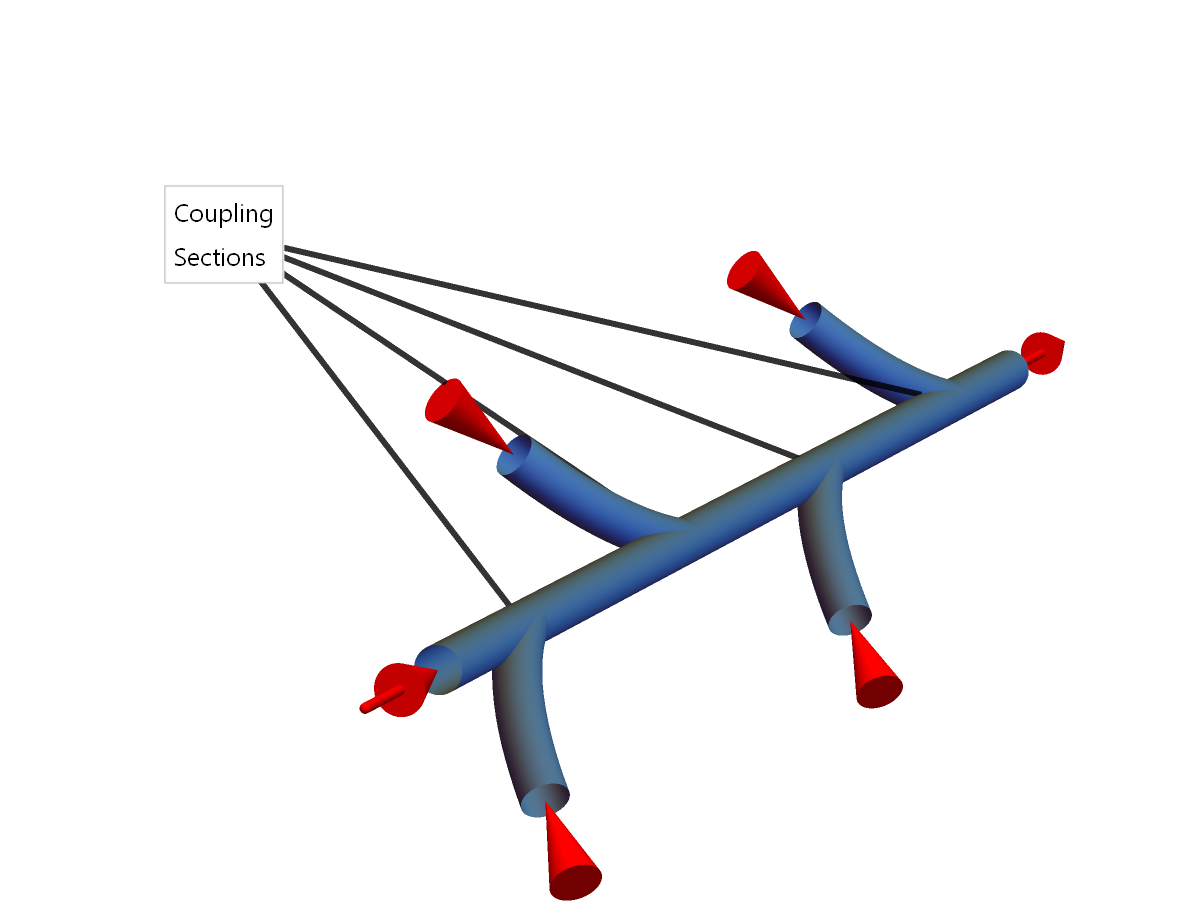
\includegraphics[width=\marginparwidth]{figures/coupling_scheme.png}
\caption{Proposed multistage acceleration scheme. The first main laser is initiating the acceleration of the electron beam. A fishbone shaped curved channels are added down the acceleration line enabling further acceleration of the electrons.}
\label{fig:coupling_scheme}
\end{marginfigure}
However, this introduces severe challenges with regard to electron beam transport in between stages \cite{Esarey2009PhysicsAccelerators}.

\end{document}